\documentclass[a4paper,12pt,reqno,oneside]{amsart}
\usepackage[T1]{fontenc}
\usepackage[utf8]{inputenc}
\usepackage{amsmath,amssymb,amsthm}
\usepackage[dvipsnames]{xcolor}
\usepackage{tikz}

\begin{document}

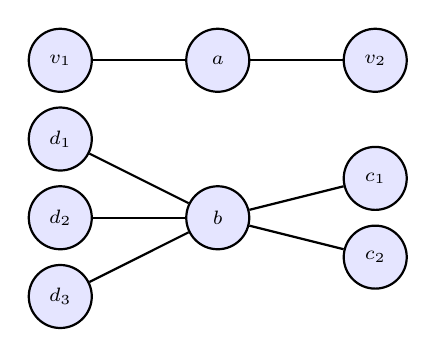
\begin{tikzpicture}[thick, main
  node/.style={circle,fill=blue!10,draw,minimum size=0.8cm,font=\sffamily\scriptsize\bfseries}]
  \node[main node] (b) at (0, 0) {$b$};
  \node[main node] (a) at (0, 2) {$a$};

  \node[main node] (v2) at ([xshift=2cm]a) {$v_2$};
  \node[main node] (v1) at ([xshift=-2cm]a) {$v_1$};

  \node[main node] (c1) at ([xshift=2cm,yshift=0.5cm]b) {$c_1$};
  \node[main node] (c2) at ([xshift=2cm,yshift=-0.5cm]b) {$c_2$};

  \node[main node] (d1) at ([xshift=-2cm,yshift=1cm]b) {$d_1$};
  \node[main node] (d2) at ([xshift=-2cm]b) {$d_2$};
  \node[main node] (d3) at ([xshift=-2cm,yshift=-1cm]b) {$d_3$};

  \draw (a) -- (v1);
  \draw (a) -- (v2);
  \draw (b) -- (d1);
  \draw (b) -- (d2);
  \draw (b) -- (d3);
  \draw (b) -- (c1);
  \draw (b) -- (c2);
\end{tikzpicture}

\end{document}